
%% bare_conf.tex
%% V1.3
%% 2007/01/11
%% by Michael Shell
%% See:
%% http://www.michaelshell.org/
%% for current contact information.
%%
%% This is a skeleton file demonstrating the use of IEEEtran.cls
%% (requires IEEEtran.cls version 1.7 or later) with an IEEE conference paper.
%%
%% Support sites:
%% http://www.michaelshell.org/tex/ieeetran/
%% http://www.ctan.org/tex-archive/macros/latex/contrib/IEEEtran/
%% and
%% http://www.ieee.org/

%%*******************************************************************:/******
%% Legal Notice:
%% This code is offered as-is without any warranty either expressed or
%% implied; without even the implied warranty of MERCHANTABILITY or
%% FITNESS FOR A PARTICULAR PURPOSE! 
%% User assumes all risk.
%% In no event shall IEEE or any contributor to this code be liable for
%% any damages or losses, including, but not limited to, incidental,
%% consequential, or any other damages, resulting from the use or misuse
%% of any information contained here.
%%
%% All comments are the opinions of their respective authors and are not
%% necessarily endorsed by the IEEE.
%%
%% This work is distributed under the LaTeX Project Public License (LPPL)
%% ( http://www.latex-project.org/ ) version 1.3, and may be freely used,
%% distributed and modified. A copy of the LPPL, version 1.3, is included
%% in the base LaTeX documentation of all distributions of LaTeX released
%% 2003/12/01 or later.
%% Retain all contribution notices and credits.
%% ** Modified files should be clearly indicated as such, including  **
%% ** renaming them and changing author support contact information. **
%%
%% File list of work: IEEEtran.cls, IEEEtran_HOWTO.pdf, bare_adv.tex,
%%                    bare_conf.tex, bare_jrnl.tex, bare_jrnl_compsoc.tex
%%*************************************************************************

% *** Authors should verify (and, if needed, correct) their LaTeX system  ***
% *** with the testflow diagnostic prior to trusting their LaTeX platform ***
% *** with production work. IEEE's font choices can trigger bugs that do  ***
% *** not appear when using other class files.                            ***
% The testflow support page is at:
% http://www.michaelshell.org/tex/testflow/



% Note that the a4paper option is mainly intended so that authors in
% countries using A4 can easily print to A4 and see how their papers will
% look in print - the typesetting of the document will not typically be
% affected with changes in paper size (but the bottom and side margins will).
% Use the testflow package mentioned above to verify correct handling of
% both paper sizes by the user's LaTeX system.
%
% Also note that the "draftcls" or "draftclsnofoot", not "draft", option
% should be used if it is desired that the figures are to be displayed in
% draft mode.
%
\documentclass[conference]{IEEEtran}
% Add the compsoc option for Computer Society conferences.
%
% If IEEEtran.cls has not been installed into the LaTeX system files,
% manually specify the path to it like:
% \documentclass[conference]{../sty/IEEEtran}
\usepackage{mathtools}
\usepackage{listings}
\usepackage{xcolor}
\usepackage{dblfloatfix}


\usepackage{float}
\usepackage{mdwlist}
\usepackage{paralist}
\usepackage{graphics}
\usepackage{enumerate}
\usepackage{dblfloatfix}

\DeclareMathSizes{9}{19}{13}{9}
\usepackage[top=1in, bottom=1in, left=1in, right=1in]{geometry}

\usepackage[FIGBOTCAP]{subfigure}

%wzp - 20150615
\usepackage{booktabs}
\usepackage{lipsum}
\usepackage{tabularx}
\usepackage{paralist}
\newcommand{\WordCapacity}{capacity}

\newcommand{\Processor}{p}
%memory
\newcommand{\WordMemory}{memory}
\newcommand{\MemoryCapacityBits}{width_{\WordMemory}}
\newcommand{\MemoryCapacity}{C_{\WordMemory}}
\newcommand{\MemoryWidth}{{width\_memory}}
%block
\newcommand{\WordDataBlockFormular}{data\_block}
\newcommand{\WordDataBlock}{data block }
\newcommand{\BlockCapacityBits}{width_block}
\newcommand{\NumberBlock}{n_{block}}
\newcommand{\DataBlockCapacity}{C_{\WordCapacity}}
%cacheline
\newcommand{\CacheLineAbbreviation}{c}
\newcommand{\CacheLineWidthBits}{width_cacheline}
\newcommand{\NumberCacheline}{n_{cacheline}}
\newcommand{\CacheLine}{cache line}
\newcommand{\CacheLineCapitalized}{Cache line}
%cache
\newcommand{\CacheCapacityAbbreviation}{cache}
\newcommand{\CacheCapacityBits}{width_cache}
\newcommand{\Associativity}{associativity }
\newcommand{\NumberSet}{n_{set}}

\newcommand{\Location}{location}
\newcommand{\SliceID}{slice\_id }
\newcommand{\WordSlice}{slice}
\newcommand{\NumberSliceID}{n_{\WordSlice}}
\newcommand{\WordSet}{set}
\newcommand{\SetIndex}{set\_index }
\newcommand{\NumberSetEachSlice}{n_{\WordSet}}
%physical address
\newcommand{\PhysicalAddress}{physical\ address}
\newcommand{\PhysicalAddressAbbreviation}{pa}
\newcommand{\findex}{ma\_to\_slice\_id}
\newcommand{\MA}{\PhysicalAddressAbbreviation}
\newcommand{\MATOSliceID}{ma\_to\_slice\_id}
\newcommand{\MATOSetIndex}{ma\_to\_set\_index}
\newcommand{\memoryaddress}{physical address}

\newcommand{\NUMSLICE}{n_{slice}}
\newcommand{\NUMSET}{n_{set}}

\newcommand{\NUMBERSLICE}{$2^{n\_slice}$}
\newcommand{\NUMBERSET}{$2^{n\_set}$}
\newcommand{\WIDTHSetIndex}{$n\_slice$}
\newcommand{\NUMBERBLOCK}{$2^{n\_block}$}
\newcommand{\WIDTHBLOCK}{$n\_block$}

\newcommand{\SandyBridge}{Sandy Bridge }
% Some very useful LaTeX packages include:
% (uncomment the ones you want to load)


% *** MISC UTILITY PACKAGES ***
%
%\usepackage{ifpdf}
% Heiko Oberdiek's ifpdf.sty is very useful if you need conditional
% compilation based on whether the output is pdf or dvi.
% usage:
% \ifpdf
%   % pdf code
% \else
%   % dvi code
% \fi
% The latest version of ifpdf.sty can be obtained from:
% http://www.ctan.org/tex-archive/macros/latex/contrib/oberdiek/
% Also, note that IEEEtran.cls V1.7 and later provides a builtin
% \ifCLASSINFOpdf conditional that works the same way.
% When switching from latex to pdflatex and vice-versa, the compiler may
% have to be run twice to clear warning/error messages.

% The following code is added by wzp to make caption of table lower case
\usepackage{etoolbox}
\makeatletter
\patchcmd{\@makecaption}
  {\scshape}
  {}
  {}
  {}
%\patchcmd{\@makecaption}
%  {\\}
%  {.\}
%  {}
%  {}
\makeatother
\def\tablename{Table}
\newcommand{\otoprule}{\midrule[\heavyrulewidth]}
%\setlength{\heavyrulewidth}{2pt}
%\setlength{\lightrulewidth}{1pt}

% *** CITATION PACKAGES ***
%
%\usepackage{cite}
% cite.sty was written by Donald Arseneau
% V1.6 and later of IEEEtran pre-defines the format of the cite.sty package
% \cite{} output to follow that of IEEE. Loading the cite package will
% result in citation numbers being automatically sorted and properly
% "compressed/ranged". e.g., [1], [9], [2], [7], [5], [6] without using
% cite.sty will become [1], [2], [5]--[7], [9] using cite.sty. cite.sty's
% \cite will automatically add leading space, if needed. Use cite.sty's
% noadjust option (cite.sty V3.8 and later) if you want to turn this off.
% cite.sty is already installed on most LaTeX systems. Be sure and use
% version 4.0 (2003-05-27) and later if using hyperref.sty. cite.sty does
% not currently provide for hyperlinked citations.
% The latest version can be obtained at:
% http://www.ctan.org/tex-archive/macros/latex/contrib/cite/
% The documentation is contained in the cite.sty file itself.






% *** GRAPHICS RELATED PACKAGES ***
%
\ifCLASSINFOpdf
  % \usepackage[pdftex]{graphicx}
  % declare the path(s) where your graphic files are
  % \graphicspath{{../pdf/}{../jpeg/}}
  % and their extensions so you won't have to specify these with
  % every instance of \includegraphics
  % \DeclareGraphicsExtensions{.pdf,.jpeg,.png}
\else
  % or other class option (dvipsone, dvipdf, if not using dvips). graphicx
  % will default to the driver specified in the system graphics.cfg if no
  % driver is specified.
  % \usepackage[dvips]{graphicx}
  % declare the path(s) where your graphic files are
  % \graphicspath{{../eps/}}
  % and their extensions so you won't have to specify these with
  % every instance of \includegraphics
  % \DeclareGraphicsExtensions{.eps}
\fi
% graphicx was written by David Carlisle and Sebastian Rahtz. It is
% required if you want graphics, photos, etc. graphicx.sty is already
% installed on most LaTeX systems. The latest version and documentation can
% be obtained at: 
% http://www.ctan.org/tex-archive/macros/latex/required/graphics/
% Another good source of documentation is "Using Imported Graphics in
% LaTeX2e" by Keith Reckdahl which can be found as epslatex.ps or
% epslatex.pdf at: http://www.ctan.org/tex-archive/info/
%
% latex, and pdflatex in dvi mode, support graphics in encapsulated
% postscript (.eps) format. pdflatex in pdf mode supports graphics
% in .pdf, .jpeg, .png and .mps (metapost) formats. Users should ensure
% that all non-photo figures use a vector format (.eps, .pdf, .mps) and
% not a bitmapped formats (.jpeg, .png). IEEE frowns on bitmapped formats
% which can result in "jaggedy"/blurry rendering of lines and letters as
% well as large increases in file sizes.
%
% You can find documentation about the pdfTeX application at:
% http://www.tug.org/applications/pdftex





% *** MATH PACKAGES ***
%
%\usepackage[cmex10]{amsmath}
% A popular package from the American Mathematical Society that provides
% many useful and powerful commands for dealing with mathematics. If using
% it, be sure to load this package with the cmex10 option to ensure that
% only type 1 fonts will utilized at all point sizes. Without this option,
% it is possible that some math symbols, particularly those within
% footnotes, will be rendered in bitmap form which will result in a
% document that can not be IEEE Xplore compliant!
%
% Also, note that the amsmath package sets \interdisplaylinepenalty to 10000
% thus preventing page breaks from occurring within multiline equations. Use:
%\interdisplaylinepenalty=2500
% after loading amsmath to restore such page breaks as IEEEtran.cls normally
% does. amsmath.sty is already installed on most LaTeX systems. The latest
% version and documentation can be obtained at:
% http://www.ctan.org/tex-archive/macros/latex/required/amslatex/math/





% *** SPECIALIZED LIST PACKAGES ***
%
%\usepackage{algorithmic}
% algorithmic.sty was written by Peter Williams and Rogerio Brito.
% This package provides an algorithmic environment fo describing algorithms.
% You can use the algorithmic environment in-text or within a figure
% environment to provide for a floating algorithm. Do NOT use the algorithm
% floating environment provided by algorithm.sty (by the same authors) or
% algorithm2e.sty (by Christophe Fiorio) as IEEE does not use dedicated
% algorithm float types and packages that provide these will not provide
% correct IEEE style captions. The latest version and documentation of
% algorithmic.sty can be obtained at:
% http://www.ctan.org/tex-archive/macros/latex/contrib/algorithms/
% There is also a support site at:
% http://algorithms.berlios.de/index.html
% Also of interest may be the (relatively newer and more customizable)
% algorithmicx.sty package by Szasz Janos:
% http://www.ctan.org/tex-archive/macros/latex/contrib/algorithmicx/




% *** ALIGNMENT PACKAGES ***
%
%\usepackage{array}
% Frank Mittelbach's and David Carlisle's array.sty patches and improves
% the standard LaTeX2e array and tabular environments to provide better
% appearance and additional user controls. As the default LaTeX2e table
% generation code is lacking to the point of almost being broken with
% respect to the quality of the end results, all users are strongly
% advised to use an enhanced (at the very least that provided by array.sty)
% set of table tools. array.sty is already installed on most systems. The
% latest version and documentation can be obtained at:
% http://www.ctan.org/tex-archive/macros/latex/required/tools/


%\usepackage{mdwmath}
%\usepackage{mdwtab}
% Also highly recommended is Mark Wooding's extremely powerful MDW tools,
% especially mdwmath.sty and mdwtab.sty which are used to format equations
% and tables, respectively. The MDWtools set is already installed on most
% LaTeX systems. The lastest version and documentation is available at:
% http://www.ctan.org/tex-archive/macros/latex/contrib/mdwtools/


% IEEEtran contains the IEEEeqnarray family of commands that can be used to
% generate multiline equations as well as matrices, tables, etc., of high
% quality.


%\usepackage{eqparbox}
% Also of notable interest is Scott Pakin's eqparbox package for creating
% (automatically sized) equal width boxes - aka "natural width parboxes".
% Available at:
% http://www.ctan.org/tex-archive/macros/latex/contrib/eqparbox/





% *** SUBFIGURE PACKAGES ***
%\usepackage[tight,footnotesize]{subfigure}
% subfigure.sty was written by Steven Douglas Cochran. This package makes it
% easy to put subfigures in your figures. e.g., "Figure 1a and 1b". For IEEE
% work, it is a good idea to load it with the tight package option to reduce
% the amount of white space around the subfigures. subfigure.sty is already
% installed on most LaTeX systems. The latest version and documentation can
% be obtained at:
% http://www.ctan.org/tex-archive/obsolete/macros/latex/contrib/subfigure/
% subfigure.sty has been superceeded by subfig.sty.



%\usepackage[caption=false]{caption}
%\usepackage[font=footnotesize]{subfig}
% subfig.sty, also written by Steven Douglas Cochran, is the modern
% replacement for subfigure.sty. However, subfig.sty requires and
% automatically loads Axel Sommerfeldt's caption.sty which will override
% IEEEtran.cls handling of captions and this will result in nonIEEE style
% figure/table captions. To prevent this problem, be sure and preload
% caption.sty with its "caption=false" package option. This is will preserve
% IEEEtran.cls handing of captions. Version 1.3 (2005/06/28) and later 
% (recommended due to many improvements over 1.2) of subfig.sty supports
% the caption=false option directly:
%\usepackage[caption=false,font=footnotesize]{subfig}
%
% The latest version and documentation can be obtained at:
% http://www.ctan.org/tex-archive/macros/latex/contrib/subfig/
% The latest version and documentation of caption.sty can be obtained at:
% http://www.ctan.org/tex-archive/macros/latex/contrib/caption/




% *** FLOAT PACKAGES ***
%
%\usepackage{fixltx2e}
% fixltx2e, the successor to the earlier fix2col.sty, was written by
% Frank Mittelbach and David Carlisle. This package corrects a few problems
% in the LaTeX2e kernel, the most notable of which is that in current
% LaTeX2e releases, the ordering of single and double column floats is not
% guaranteed to be preserved. Thus, an unpatched LaTeX2e can allow a
% single column figure to be placed prior to an earlier double column
% figure. The latest version and documentation can be found at:
% http://www.ctan.org/tex-archive/macros/latex/base/



%\usepackage{stfloats}
% stfloats.sty was written by Sigitas Tolusis. This package gives LaTeX2e
% the ability to do double column floats at the bottom of the page as well
% as the top. (e.g., "\begin{figure*}[!b]" is not normally possible in
% LaTeX2e). It also provides a command:
%\fnbelowfloat
% to enable the placement of footnotes below bottom floats (the standard
% LaTeX2e kernel puts them above bottom floats). This is an invasive package
% which rewrites many portions of the LaTeX2e float routines. It may not work
% with other packages that modify the LaTeX2e float routines. The latest
% version and documentation can be obtained at:
% http://www.ctan.org/tex-archive/macros/latex/contrib/sttools/
% Documentation is contained in the stfloats.sty comments as well as in the
% presfull.pdf file. Do not use the stfloats baselinefloat ability as IEEE
% does not allow \baselineskip to stretch. Authors submitting work to the
% IEEE should note that IEEE rarely uses double column equations and
% that authors should try to avoid such use. Do not be tempted to use the
% cuted.sty or midfloat.sty packages (also by Sigitas Tolusis) as IEEE does
% not format its papers in such ways.





% *** PDF, URL AND HYPERLINK PACKAGES ***
%
%\usepackage{url}
% url.sty was written by Donald Arseneau. It provides better support for
% handling and breaking URLs. url.sty is already installed on most LaTeX
% systems. The latest version can be obtained at:
% http://www.ctan.org/tex-archive/macros/latex/contrib/misc/
% Read the url.sty source comments for usage information. Basically,
% \url{my_url_here}.





% *** Do not adjust lengths that control margins, column widths, etc. ***
% *** Do not use packages that alter fonts (such as pslatex).         ***
% There should be no need to do such things with IEEEtran.cls V1.6 and later.
% (Unless specifically asked to do so by the journal or conference you plan
% to submit to, of course. )


% correct bad hyphenation here
\hyphenation{op-tical net-works semi-conduc-tor}

\begin{document}
%
% paper title
% can use linebreaks \\ within to get better formatting as desired
\title{\huge{\textbf{A Summary of the Development of AI in Go Playing Area}}}


% author names and affiliations
% use a multiple column layout for up to three different
% affiliations
\author{
%\IEEEauthorblockN{Michael Shell}
%\IEEEauthorblockA{School of Electrical and\\Computer Engineering\\
%Georgia Institute of Technology\\
%Atlanta, Georgia 30332--0250\\
%Email: http://www.michaelshell.org/contact.html}
%\and
%\IEEEauthorblockN{Homer Simpson}
%\IEEEauthorblockA{Twentieth Century Fox\\
%Springfield, USA\\
%Email: homer@thesimpsons.com}
%\and
%\IEEEauthorblockN{James Kirk\\ and Montgomery Scott}
%\IEEEauthorblockA{Starfleet Academy\\
%San Francisco, California 96678-2391\\
%Telephone: (800) 555--1212\\
%Fax: (888) 555--1212}

%\IEEEauthorblockN{Zhipeng Wei}
%\IEEEauthorblockA{weizhipeng@ict.ac.cn}
%\and
%\IEEEauthorblockN{Zehan Cui}
%\IEEEauthorblockA{cuizehan@ict.ac.cn}
%\and
%\IEEEauthorblockN{Mingyu Chen}
%\IEEEauthorblockA{cmy@ict.ac.cn}

\IEEEauthorblockN{Zhipeng Wei}
%\IEEEauthorblockA{\\Insitute of Computing Technology, Chinese Academy of Sciences \\ $\left\{weizhipeng, cuizehan, cmy\right\}$@ict.ac.cn}
}
% conference papers do not typically use \thanks and this command
% is locked out in conference mode. If really needed, such as for
% the acknowledgment of grants, issue a \IEEEoverridecommandlockouts
% after \documentclass

% for over three affiliations, or if they all won't fit within the width
% of the page, use this alternative format:
% 
%\author{\IEEEauthorblockN{Michael Shell\IEEEauthorrefmark{1},
%Homer Simpson\IEEEauthorrefmark{2},
%James Kirk\IEEEauthorrefmark{3}, 
%Montgomery Scott\IEEEauthorrefmark{3} and
%Eldon Tyrell\IEEEauthorrefmark{4}}
%\IEEEauthorblockA{\IEEEauthorrefmark{1}School of Electrical and Computer Engineering\\
%Georgia Institute of Technology,
%Atlanta, Georgia 30332--0250\\ Email: see http://www.michaelshell.org/contact.html}
%\IEEEauthorblockA{\IEEEauthorrefmark{2}Twentieth Century Fox, Springfield, USA\\
%Email: homer@thesimpsons.com}
%\IEEEauthorblockA{\IEEEauthorrefmark{3}Starfleet Academy, San Francisco, California 96678-2391\\
%Telephone: (800) 555--1212, Fax: (888) 555--1212}
%\IEEEauthorblockA{\IEEEauthorrefmark{4}Tyrell Inc., 123 Replicant Street, Los Angeles, California 90210--4321}}




% use for special paper notices
%\IEEEspecialpapernotice{(Invited Paper)}




% make the title area
\maketitle



% IEEEtran.cls defaults to using nonbold math in the Abstract.
% This preserves the distinction between vectors and scalars. However,
% if the conference you are submitting to favors bold math in the abstract,
% then you can use LaTeX's standard command \boldmath at the very start
% of the abstract to achieve this. Many IEEE journals/conferences frown on
% math in the abstract anyway.

% no keywords

% For peer review papers, you can put extra information on the cover
% page as needed:
% \ifCLASSOPTIONpeerreview
% \begin{center} \bfseries EDICS Category: 3-BBND \end{center}
% \fi
%
% For peerreview papers, this IEEEtran command inserts a page break and
% creates the second title. It will be ignored for other modes.
\IEEEpeerreviewmaketitle

\input{abstract}
\input{introduction}
\section{background knowledge}
\subsection{Neural network}
\subsubsection{history}
In machine learning and cognitive science, artificial neural networks (ANNs) are a family of models inspired by biological neural networks (the central nervous systems of animals, in particular the brain) and are used to estimate or approximate functions that can depend on a large number of inputs and are generally unknown. Artificial neural networks are generally presented as systems of interconnected "neurons" which exchange messages between each other. The connections have numeric weights that can be tuned based on experience, making neural nets adaptive to inputs and capable of learning.

For example, a neural network for handwriting recognition is defined by a set of input neurons which may be activated by the pixels of an input image. After being weighted and transformed by a function (determined by the network's designer), the activations of these neurons are then passed on to other neurons. This process is repeated until finally, an output neuron is activated. This determines which character was read.

Like other machine learning methods – systems that learn from data – neural networks have been used to solve a wide variety of tasks that are hard to solve using ordinary rule-based programming, including computer vision and speech recognition.

\textbf{summary:}it's a simulation of human neural network, it's used to perform some tasks. For example, in the field of character recognizing, the pixels of the image serve as input. The output should indicate which character the character is.
\subsection{Machine learning}
Machine learning is a subfield of computer science that evolved from the study of pattern recognition and computational learning theory in artificial intelligence. It's defined as a "field of study that gives computers the ability to learn without explicitly programmed". Machine learning explores the study and construction of algorithms that can learn from and make predictions on data. Such algorithms operate by \textbf{building model from example inputs in order to make data-driven predictions or decisions}, rather than following strictly static program instructions.
\subsection{Deep learning}
Deep learning (deep structured learning, hierarchical learning or deep machine learning) is a branch of machine learning based on a set of algorithms that attempt to model high-level abstractions in data by using multiple processing layers, with complex structures or otherwise, composed of multiple non-linear transformations.


\section{related work}
The section lists the main ideas of the papers the author has read. In order to show the evolution of the technology, those papers are organized in chronological order.
\subsection{Monte Carlo Go paper 1993~\cite{brugmann1993monte, silver2009monte, browne2012survey}}
\subsubsection{Abstract}
This paper present an algorithm for the board game go which attempts to find the best move by simulated 
annealing. Using this method, without including any go knowledge beyond the rules, this paper manages
to a playing strength of about 25 kyu on a $9\times9$ board.
\subsubsection{Introduction}
The author started the discussion using "how would nature play go?" Then the author tried to use simulated 
annealing to solve the problem. The basic idea of the method is simple: 
\begin{inparaenum}
	\item moves are performed randomly with probabilities assigned by the method of simulated annealing;
	\item the value of a position in which the game is over is defined by counting, and 
	\item to find the best move in a given position play the game to the very end as suggested by (i) 
		and then evaluate as in (2); play many such random games, and the best move will be the one which does best on average.
\end{inparaenum}
The author also believes that the idea is simple, and any good idea can be stated simply. In this paper, the authors also tried to convince the readers that this is at least not a bad idea.
\subsubsection{Simulated annealing for mathematical problems}
If you want to find the minimum of one function, if the function is simple enough and depends only on a small number of variables, there are very efficient exact numerical methods to find its local minima. They are all based essentially the same principle. Pick initial values for each variable and compute the function. Change the variables slightly in such a way that the function velue decreases. Repetition allows one to come arbitrarily close to a local minimum. Different algorithms have been invented to optimize the process at each iteration for different classes of functions.

There are several types of problems where there is virtually no alternative to simulated annealing. As it turns out, these exact algorithms are greedy by design, that is given a starting point they greedily walk downhill (following the steepest descent) until they have found a local minimum. But if one is looking for a global minimum among many local ones, and if one does not know before-hand where to look for it, one will never find it.

Two combinatorial optimization, traveling salesman problem. These problems are examples for combinatorial optimization since the configuration space on which function is to be minimized is a discrete, factorially large space. In the traveling salesman problem, there are $N = N \times (N-1) \times \times 1$ possibilities to make an ordered list of N cities.

Second example is to find the arrangement of 25 playing cards in a $5 \times 5$ tableau such that the value of the rows, columns, and diagonals interpreted as hands for poker is maximized.
\subsection{Probabilistic reasoning over time}
In which we try to interpret the present, understand the past, and perhaps predict the future, even when very little is crystal clear.
\subsubsection{Time and uncertainty}
Two cases, car repair, we assume that whatever is broken remains broken during the process of diagnosis; our job is to refer the state of the car from observed evidence.
%\subsubsection{Inference in temporal model}
%\textbf{Filtering:} this is the task of computing the belief state - the posterior distribution ove the most recent state - given all evidence to date. Filtering is also called state estimation. This is what a rational agent does to keep track of the current state so that rational decisions can be made.
%\textbf{prediction:} this is the task of computing the posterior distribution over the future state, given all evidence to date. This is used to calculate the probability distribution of future events.
%\textbf{smoothing:}
%\textbf{Most likely explanation:}
%\subsubsection{SmartGame library}
%The SMARTGAME library contains generally useful game-independent functionality. It includes utility classes, classes that encapsulate non-portable platform-dependent functionality, and classes and functions that help to represent the game state for two-player games on square boards.
\subsection{Fuego software framework~\cite{enzenberger2010fuego}}
FUEGO, as an open source software framework, can facilitate and accelerate research. 
It's able to play the game of Go. The framework supports developing game engines for full-information two-player 
board games, and is used successfully in a substantial number of projects. The FUEGO 
Go program became the first program to win a game against a top professional player in $9 \times 9$ Go.
Advance in theory, such as MCTS and the UCT algorithm have led to breakthrough performance in computer Go.
% This is a paper in 2015 
\subsection{Move evaluation in go using deep convolutional neural networks~\cite{maddison2014move, clark2015training}}
The game of Go is more challenging than other board games, due to difficulty of constructing a position or move evaluation function. This paper investigates whether deep convolutional networks can be used to directly represent and learn this knowledge. The paper trains a 12-layer convolutional neural network by supervised learning from a database of human professional games. The network correctly predicts the expert move in 55\% of positions, equaling the accuracy of a 6 dan human player.

The contributions of thie paper lie in the following aspects. Although CNNs have previously been applied to the game of Go, with modest success, previous architectures have typically been limited to one hidden layer of relatively small size, and have not exploited recent advances in computational power. This paper uses deeper and larger CNNs of 12 hidden layers and several billion connections to represent and learn knowledge. And this increase in depth and size leads to a qualitative jump in performance, suggesting that contrary to previous beliefs, a strong move evaluation function for Go can indeed be represented and learnt by such architectures.

Convolutional neural networks have a long history in the game of Go. Schraudolph Schraudolph
et al. (1994) trained a simple CNN (exploiting rotational, reflectional, and colour inversion symmetries)
to predict final territory, by reinforcement learning from games of self-play. The resulting
program beat a simplistic handcrafted program called Wally. NeuroGo (Enzenberger, 1996) used
a more sophisticated architecture to predict final territory, eyes, and connectivity, again exploiting
symmetries; and used a connectivity pathfinder to propagate information across weakly connected
groups of stones. Enzenberger's program also used reinforcement learning from self-play. When
combined with an alpha-beta search, NeuroGo equalled the performance of GnuGo on 9 $\times$ 9 Go,
and reached around 13 kyu on 19$\times$19 Go. Sutskever \& Nair (2008) applied convolutional networks
to supervised learning of expert moves, but using a small 1 hidden layer CNN; this matched
the state-of-the-art prediction performance, achieving 34.6\% accuracy, but this was not sufficient to
play Go at any reasonable level.

The 12 layer neural network has implicitly understood many sophisticated aspects of Go, including good
shape (patterns that maximise long term effectiveness of stones), Fuseki (opening sequences), Joseki
(corner patterns), Tesuji (tactical patterns), Ko fights (intricate tactical battles involving repeated
recapture of the same stones), territory (ownership of points), and influence (long-term potential
for territory). It is remarkable that a single, unified, straightforward architecture can master these
elements of the game to such a degree, and without any explicit lookahead.

It appears that we now have two core elements that scale effectively with increased computational resources: scalable planning, using Monte-Carlo search; and scalable evaluation functions, using deep neural netowrks. In the future, as parallel computation units such as GPUs continue to increase in performance, we believe that this trajectory of research will lead to considerably stronger programs than are currently possible.

The method might work well, but it also has its own weakness. Notably it sometimes fails to understand the global picture, behaving as if the life and death status of large groups has been incorrectly assessed. Interestingly, it is precisely these global aspects of the game for which Monte-Carlo search excels, suggesting that these two techniques may be largely complementary. We have provided a preliminary proof-of-concept that MCTS and deep neural networks may be combined effectively.
% Facebook paper
\subsection{Better Computer go player with neural network and long-term prediction~\cite{tian2015better, schaeffer2001temporal}}
This work is done by some researchers at Facebook.
\subsubsection{Abstract}
Search is not strictly necessary for machine Go players. A pure pattern-matching approach, based on a deep convolutional neural network that predicts the next move, can perform as well as Monte Carlo Tree Search-based open source Go engine such as Pachi if its search budget is limited.

Darkforest relies on a DCNN designed for long-term predictions. While the previous methods can predict the next move that a human would play 55.2\% of the time. However, whether this accuracy leads to a strong Go AI is not yet well understood. This paper tries to show that DCNN-based move predictions indeed give a strong Go AI, if properly trained.
\subsubsection{Introduction}
Recent study shows that the Go board situation could be deciphered with Deep Convolutional Neural Network. They can predict the next move that a human would play 55.2\% of the time. In this paper, the authors show that DCNN-based move predictions indeed give a strong Go AI, if properly trained. In particular, the authors carefully design the training process and choose to predict next k moves rather than the immediate next move to enrich the gradient signal.
%
%What kind of data is used to train?
%\subsubsection{method}
%\subsubsection{feature channel}
\subsubsection{Network architecture}
This paper uses a 12-layered full convolutional network. Each convolutional layer is followed by a ReLU 
nonlinearity. Except for the first layer, all layers use the same width w = 384. No weight sharing is used. 
We do not use pooling since they negatively affect the performance. Instead of using two softmax outputs to 
predict black and white moves, we only use one softmax layer to predict the next move, reducing the number 
of parameters.
\subsubsection{Long term planning}
Predicting only the immediate next move limits the informaiton received by the lower layers. Instead, we 
predict next k moves from the current board situation. Each move is a separate softmax output. The motivation
is two-fold. First, we want our network to focus on a strategic plan rather than the immediate next move. 
Second, with multiple softmax outputs, we expect to have more supervisions to train the network. 
\subsubsection{Training}
When training, we use 16 CPU threads to prepare the minibatch, each simulating 300 random selected
games from the dataset. In each minibatch, for each thread, randomly select one game out of
300, simulate one step according to the game record, and extract features and next k moves as the
input/output pair in the batch. If the game has ended (or fewer than k moves are left), we randomly
pick one (with replacement) from the training set and continue. The batch size is 256. We use data
augmentation with rotation at 90-degree intervals and horizontal vertical flipping. For each board
situation, data augmentation could generate up to 8 different situations.
Before training, we randomly initialize games into different stages. This ensures that each batch
contains situations corresponding to different stages of games. Without this, the network will quickly
overfit and get trapped into poor local minima.
\subsubsection{Monte carlo tree search}
From the experiments, we clearly show that DCNN is tactically weak due to the lack of search.
Search is a way to explore the solution space conditioned on the current board situation, and build
a non-parametric local model for the game. The local model is more flexible than the global model
learned from massive training data and more adapted to the current situation. The state-of-the-art
approach in computer Go is Monte-Carlo Tree Search (MCTS).
%\subsubsection{Knowledge representation}
%The author tries to give the definition of what knowledge is. Something is strange that this question has never been answered directly. In history, different people have tried to describe it from different prospectives. The authors believe that this question can be answered in terms of five important and distinctly different roles that a representation play.
%\begin{enumerate}
%	\item A knowledge representation is most fundamentally a surrogate, a substitute for the thing itself, used to enable an entity to determine consequences by thinking rather than acting;
%	\item It is a set of ontological commitments;
%	\item It's a fragmentary theory of intelligent reasoning;
%	\item It's a medium for pragmatically efficient computation;
%	\item It's a medium of human expression.
%\end{enumerate}
%Also there are two terminologies, inference, to mean any way to get new expressions from old; give the familiar set of basic representation tools like logic, rule, frames, semantic nets, as knowledge representation technologies.
\subsection{Bayesian Pattern Ranking for Move Prediction in the game of Go~\cite{stern2006bayesian}}
This paper, the authors investigate the problem of learning to predict moves in the board game of Go from game records of expert players. They obtain a probability distribution over legal moves for professional play in a given position.
This distribution can be quite useful, it can serve as a stand-alone player; and it can also be a move selector and move sorter. Two major components: a pattern extraction scheme for efficiently harvesting patterns of given size and shape from expert game; a Bayesian learning algorithm that learns a distribution ove the values of a move given a board position based on hte local pattern context.

Go has emerged as a major challenge for AI with the best computer Go programs currently playing at the level of weak amateur human players. This stands in stark contrast with the state of computer chess where computers play beyond human world class level. In Go, global search is typically replaced with a hybrid of local search, pattern matching and territory estimation.
%\subsubsection{board and pattern representation}
%how to represent a board configuration and the properties of these patterns;
%\subsubsection{local features}
%
%\subsubsection{pattern matching and storing}
%\subsubsection{pattern harvesting}
%\subsubsection{models for move prediction}
%
\subsection{Mimicking Go Experts with Convolutional Neural Networks~\cite{sutskever2008mimicking}}
\subsubsection{The techniques useful for chess are not useful for Go}
First, the nature of the rules of Chess makes it easy to estimate the player with the advantage, simply by counting the pieces. This and similar heuristics allow minimax search to compute a good move reasonably rapidly. In contrast, there is no easy way to determine the player with the advantages in Go. In particular, counting captured pieces does not work for Go because the value of a piece depends more heavily on its surroundings. The ability to raplidly evaluate Go positions prevents minimax searches from finding good moves. Second, typical Chess positions have 40 legal moves, while typical Go positions have 200 legal moves, so the search space is substantially larger. This partly explains why there are still no strong computer Go players.
\subsubsection{Move predictor}
Constructing a fairly accurate move predictor is potentially easier than playing Go well, because an accurate move predictor can occasionally make devastating mistakes which would make it a poor Go player.
\subsection{Mastering the game of Go with deep neural networks and tree search~\cite{silver2016mastering}}
All game of perfect inforamtion has a optimal value function, which determines the outcome of the game. Two factors deterimines the the complexity of the game, braching factor and depth. To improve the performance, the effective search space can be reduced by two general principles. First, the depth of the search may be reduced by position evaluation: truncating the search space at state s and replacing the subtree below s by an approapriate value function that predicts the outcome from state s; Second, the breadth of the search may be reduced by sampling actions from a policy p(a|s) that is a probability distribution over possible moves a in position s. As discussed above, the search space of Go is too large, so it is not possible to traverse the whole space to get the final result. The basic idea is, use the old methods, but combine them. 
\begin{figure*}[!ht]
  \caption{The complexity comparison of different board games}
  \centering
    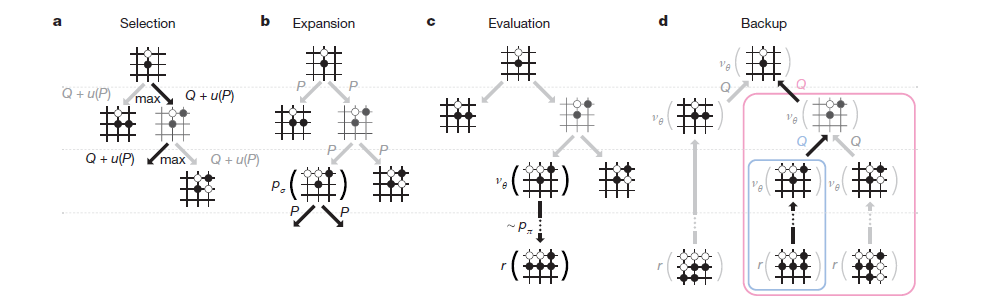
\includegraphics[width=0.9\textwidth]{MCTS-AlphaGo.png}
\end{figure*}
To address this problem, these researchers propose to solve the problem using two parts, policy network and value network. It's trained using supervised learning and reinforcement learning.

The policy network is to imitate the bahaviors of human. Given the current state of the board, the network will return some promising-looking moves. And these information is fed into the value network. The value network will evaluate these moves basically based on the previous games.
\begin{figure*}[!ht]
  \caption{Alpha Go training pipeline.}
  \centering
    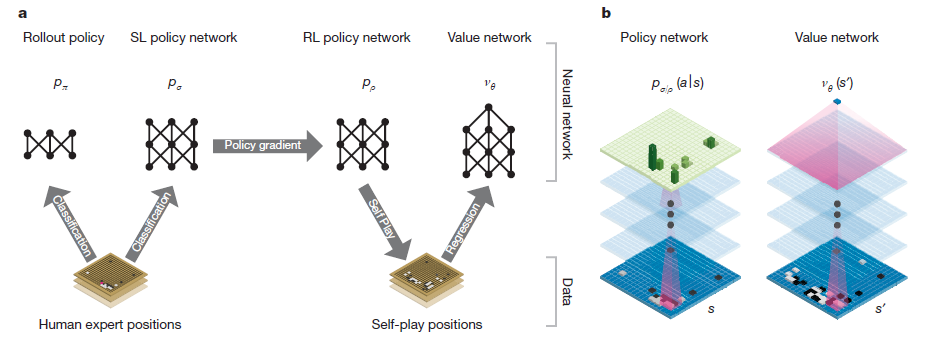
\includegraphics[width=0.9\textwidth]{AlphaGoTrainingPipeline.png}
\end{figure*}
\subsubsection{Supervised learning of policy networks}
This is the first stage of the training pipeline. The training is performed on 30 million positions from the KGS Go Server. The result is a 13 layer policy network
\subsubsection{Reinforcement learning of policy networks}
The second stage of the training pipeline aims at improving the policy network by policy gradient reinforcement learning.
\subsubsection{Reinforcement learning of value networks}
Ideally, we would like to know the optimal value function under perfect play; in practice, we instead estimate the value function for our strongest policy.
\subsubsection{Seaerching with policy and value networks}

\subsubsection{Evaluating the playing strength of AlphaGo}
To evaluate AlphaGo, a single machine version and a distributed version are used:
\begin{inparaenum}
	\item Single machine AlphaGo is many dan ranks stronger than any previous Go program. To provide a greater challenge to AlphaGo, the author also played games with four handicap stones; AlphaGo won 77\%, 86\%, and 99\% of handicap games against Crazy Stone, Zen and Pachi, respectively. The distributed version of AlphaGo was significantly stronger, winning 77\% of games against single-machine AlphaGo and 100\% of its games against other programs;
	\item The distributed version is evaluated against Hui Fan;
\end{inparaenum}
\subsubsection{Discussion}
Deep learning is based on two things: plenty of processing grunt and large amount of data. DeepMind trained its machine on a sample of 30m Go positions culled from online servers where amateurs and professionals gather to play. And by having AlphaGo play against another, slightly tweaked version of itself, more training data can be generated quickly.

How many hardware resources are there? The version playing against Mr Lee uses 1920 standard processor chips and 280 special ones developed originally to produce graphics for video games. At least part of the reason AlphaGo is ahead of the competition is that it runs on more potent hardware.

Go is exemplary in many ways of the difficulties faced by artificial inteligence: a challenge decision-making task, an intractable search space, and an optimal solution so complex it appears infeasible to directly approximate using a policy or value function. The previous major breakthough in computer Go, the introduction of MCTS, led to corresponding advances in many other domains; for example, general game-playing, classical planning, partially observed planning, scheduling, and constraint satisfaction.

Why is it meaningful? The techniques employed in AlphaGo can be used to teach computers to recognize faces, translate between languages, show relevant advertisements to internet users or hunt for subatomic particles in data from atom-smashers. Deep learning is thus a booming business. It powers the increasingly effective image- and voice-recognition abilities of computers, and firms such as Google, Facebook and Baidu are throwing money at it.

In summary, AlphaGo's success can largely be traced to a combination of the following two powerful technologies: 
\begin{inparaenum}
\item Monte Carlo tree search, this involves choosing moves at random and then simulating the game to the very end to find a winning strategy;
\item Deep reinforcement learning, a multi-layered neural network that mimics brain connections, which contains of a "policy network" that selects the next move and a "value network" that predicts the winner of the game. But there is a missing piece, the ability to learn how the world works - such as understanding the laws of physics, and the consequence of one's actions.
\end{inparaenum}
These methods have spanned a long time in the history. They appear in different background. 

%To answer the queation, the more accurate statement is that everyone believed that without some fundamentally new ideas about the structure of Go or its play, computers would never challenge Go masters. People talk about pattern recognition, but never seem to find the right ideas.

As pointed out in this paper~\cite{maddison2014move}, neural network sometimes has its weakness: it sometimes fails to understand the gobal picture, behaving as if the life and death status of large groups would be incorrectly assessed. However, Monte Carlo method can excel in these aspects. If these method were combind, good results are achieved.


\section{Comparison}
These methods have spanned a long time in the history. They appear in different background. 
\subsection{Limitations of different methods}
\subsection{Open problems}

\section{background}

%\begin{table}
%	\centering
%	\begin{tabular}{cccc}
%		\toprule
%		stride  &number    & stride & number \\ \otoprule
%		64B      & $15 \times 2^{14}$  &   32KB      &   $15 \times 2^{5}$     \\ \midrule
%		128B     & $15 \times 2^{13}$  &   64KB      &   $15 \times 2^{4}$     \\ \midrule
%		256B     & $15 \times 2^{12}$  &  128KB      &   $15 \times 2^{3}$     \\ \midrule
%		512B     & $15 \times 2^{11}$  &  256KB      &   $15 \times 2^{3}$     \\ \midrule
%		 1KB     & $15 \times 2^{10}$  &  512KB      &   $15 \times 2^{3}$     \\ \midrule
%		 2KB     & $15 \times 2^{9}$   &    1MB      &   $15 \times 2^{3}$     \\ \midrule
%		 4KB     & $15 \times 2^{8}$   &    2MB      &   $15 \times 2^{3}$     \\ \midrule
%		 8KB     & $15 \times 2^{7}$   &    4MB      &   $15 \times 2^{3}$     \\ \midrule
%		16KB     & $15 \times 2^{6}$   &    8MB      &   $15 \times 2^{3}$     \\ \bottomrule
%		\end{tabular}
%		\caption{The number of cache lines that reside in cache when accessing using different stride and array size.}
%		\label{table:3bitscombinationshuffled}
%\end{table}
%\subsection{Cache capacity per color}
%When ULCC has been ported to Sandy Bridge processor, this article implement a program to see whether we can specify the cache capacity can use through page coloring. The main function of the program is allocating a segment of memory and perform sequential accessing. By changing the size of physical memory sequentially accessed and specifying the color of physical memory can use, when the size of accessed physical memory exceeds the size of the specified cache capacity, the difference will be indicated by average access latency. 
%\begin{figure*}
%\centering
%\subfigure[Figure A]{
%		\includegraphics[width=3in]{one_color_size_without_with.eps}
%		\label{fig:subfigure1}
%	}
%	~
%	\subfigure[Figure B]{
%		\includegraphics[width=3in]{two_color_size_without_with.eps}
%		\label{fig:subfigure2}
%	}
%        ~
%        \subfigure[Figure C]{
%		\includegraphics[width=3in]{three_color_size_without_with.eps}
%		\label{fig:subfigure3}
%	}
%	~
%	\subfigure[Figure D]{
%		\includegraphics[width=3in]{four_color_size_without_with.eps}
%		\label{fig:subfigure3}
%	}
%	\caption{The capacity of each four with ULCC support with the cracked hash function support.}
%	\label{fig:CacheSizeEachColor}
%\end{figure*}
%
%On Intel Sandy Brige 4 core processor, each cache color corresponds to 80KB cache capacity. With the number of colors specifed, the cache capacity the testing program can use is restricted. When the size of accessed memory is exceeds the cache capacity the program can use, severe cache conflict will happen and average access latency will incrase. 
%
%As presented in figure~\ref{fig:CacheSizeEachColor}, implement ULCC based the cracking result of Sandy Bridge 4 core hash function. With number of cache colors specified as 1, 2, 3 and 4, the exact cache size the testing program uses is refected clearly by the cache size when the average access latency increases sharply. 
% An example of a floating figure using the graphicx package.
% Note that \label must occur AFTER (or within) \caption.
% For figures, \caption should occur after the \includegraphics.
% Note that IEEEtran v1.7 and later has special internal code that
% is designed to preserve the operation of \label within \caption
% even when the captionsoff option is in effect. However, because
% of issues like this, it may be the safest practice to put all your
% \label just after \caption rather than within \caption{}.
%
% Reminder: the "draftcls" or "draftclsnofoot", not "draft", class
% option should be used if it is desired that the figures are to be
% displayed while in draft mode.
%
%\begin{figure}[!t]
%\centering
%\includegraphics[width=2.5in]{1.eps}
% where an .eps filename suffix will be assumed under latex, 
% and a .pdf suffix will be assumed for pdflatex; or what has been declared
% via \DeclareGraphicsExtensions.
%\caption{Simulation Results}
%\label{fig_sim}
%\end{figure}

% Note that IEEE typically puts floats only at the top, even when this
% results in a large percentage of a column being occupied by floats.


% An example of a double column floating figure using two subfigures.
% (The subfig.sty package must be loaded for this to work.)
% The subfigure \label commands are set within each subfloat command, the
% \label for the overall figure must come after \caption.
% \hfil must be used as a separator to get equal spacing.
% The subfigure.sty package works much the same way, except \subfigure is
% used instead of \subfloat.
%
%\begin{figure*}[!t]
%\centerline{\subfloat[Case I]\includegraphics[width=2.5in]{subfigcase1}%
%\label{fig_first_case}}
%\hfil
%\subfloat[Case II]{\includegraphics[width=2.5in]{subfigcase2}%
%\label{fig_second_case}}}
%\caption{Simulation results}
%\label{fig_sim}
%\end{figure*}
%
% Note that often IEEE papers with subfigures do not employ subfigure
% captions (using the optional argument to \subfloat), but instead will
% reference/describe all of them (a), (b), etc., within the main caption.


% An example of a floating table. Note that, for IEEE style tables, the 
% \caption command should come BEFORE the table. Table text will default to
% \footnotesize as IEEE normally uses this smaller font for tables.
% The \label must come after \caption as always.
%
%\begin{table}[!t]
%% increase table row spacing, adjust to taste
%\renewcommand{\arraystretch}{1.3}
% if using array.sty, it might be a good idea to tweak the value of
% \extrarowheight as needed to properly center the text within the cells
%\caption{An Example of a Table}
%\label{table_example}
%\centering
%% Some packages, such as MDW tools, offer better commands for making tables
%% than the plain LaTeX2e tabular which is used here.
%\begin{tabular}{|c||c|}
%\hline
%One & Two\\
%\hline
%Three & Four\\
%\hline
%\end{tabular}
%\end{table}


% Note that IEEE does not put floats in the very first column - or typically
% anywhere on the first page for that matter. Also, in-text middle ("here")
% positioning is not used. Most IEEE journals/conferences use top floats
% exclusively. Note that, LaTeX2e, unlike IEEE journals/conferences, places
% footnotes above bottom floats. This can be corrected via the \fnbelowfloat
% command of the stfloats package.
%\section{Conclusion}
%The conclusion goes here.






% use section* for acknowledgement
%\section*{Acknowledgment}
%
%
%The authors would like to thank...





% trigger a \newpage just before the given reference
% number - used to balance the columns on the last page
% adjust value as needed - may need to be readjusted if
% the document is modified later
%\IEEEtriggeratref{8}
% The "triggered" command can be changed if desired:
%\IEEEtriggercmd{\enlargethispage{-5in}}

% references section

% can use a bibliography generated by BibTeX as a .bbl file
% BibTeX documentation can be easily obtained at:
% http://www.ctan.org/tex-archive/biblio/bibtex/contrib/doc/
% The IEEEtran BibTeX style support page is at:
% http://www.michaelshell.org/tex/ieeetran/bibtex/
%\bibliographystyle{IEEEtran}
% argument is your BibTeX string definitions and bibliography database(s)
%\bibliography{IEEEabrv,../bib/paper}
%
% <OR> manually copy in the resultant .bbl file
% set second argument of \begin to the number of references
% (used to reserve space for the reference number labels box)
%\begin{thebibliography}{1}
%
%\bibitem{IEEEhowto:kopka}
%H.~Kopka and P.~W. Daly, \emph{A Guide to \LaTeX}, 3rd~ed.\hskip 1em plus
%  0.5em minus 0.4em\relax Harlow, England: Addison-Wesley, 1999. 
%\end{thebibliography}

\bibliographystyle{abbrv}
\bibliography{IEEEexample}

% that's all folks
\end{document}


